%
% Clases de módulo de TKR.
% Análisis y diseño de programa tokenizador, reporte técnico.
%
% Proyecto Lovelace.
%

\subsubsection{Clases de TKR}
\label{sec:tkr_disenio}

En la figura \ref{clases_tkr} se muestran las clases relacionadas al módulo de
TKR. Al igual que con el diagrama anterior, la gran mayoría de las clases
pertenecen al paquete de implementaciones; las excepciones marcan el paquete al
que pertenecen.

Este es el primer diagrama en donde es necesario mostrar el esquema de acceso a
una fuente de datos. Este es descrito por una interfaz llamada CDV
(\acrlong{gl:cdv}), que define las operaciones que debe de proveer cualquier
fuente de datos que se desee usar dentro del programa. En un primer esquema
existen dos clases concretas que implementan esta interfaz: un acceso trivial y
un acceso a MySQL (ver sección \ref{sec:tecnologias}). El acceso trivial permite
definir métodos «de prueba» cuando se introduce una nueva operación en la
interfaz; de esta forma, el código cliente puede ocupar esta implementación en
lo que se desarrolla la verdadera, con conexión a base de datos. Esta manera de
separar interfaz de implementación para el acceso a datos es un patrón de
arquitectura conocido como \gls{gl:dao}; a grandes rasgos permite separar la
definición de \textit{qué} datos necesita la aplicación, del \textit{cómo} los
obtendrá; de esta manera, un cambio en el gestor de base de datos no debe
afectar al código que usa la interfaz.

En la parte inferior del diagrama se muestra la clase \textit{Registro}. Esta
representa la única clase de datos del entorno del modelo; contiene la relación
entre un \gls{gl:pan} y un \gls{gl:token}. Como aclaración, es la única clase de
datos del modelo del módulo del programa tokenizador; la interfaz web
introducirá muchas otras clases al modelo.

TKR, como se explicó en la sección \ref{sec:tkr}, necesita de una función que
genere tokens pseudoaleatorios (la función RN) la cuál necesita de una función
proveedora de bits pseudoaleatorios. En el diagrama se muestran tres versiones
de esta última función: una trivial, una basada en \gls{gl:aes} y la tercera
basada en un \gls{gl:drbg} (costado izquierdo del diagrama). La trivial es una
primera implementación que genera números pseudoaleatorios de un modo que no es
criptográficamente seguro. La basada en \gls{gl:aes} es tal cuál se decribe en
el artículo \cite{doc_sandra}. Por último, la basada en un \gls{gl:drbg},
es la que permite definir el algoritmo tokenizador que se describe en la sección
\ref{sec:drbg_lista}; para este algoritmo se ocupa la misma estructura que para
TKR, sin embargo, lo que importa en esta implementación es la propia creación
del generador, que se muestra en secciones posteriores.

La relación entre la función RN y su mecanismo de generación interno está
totalmente desacoplada: lo único que necesita la clase de la función RN es otra
función que reciba enteros sin signo y entregue arreglos de bytes. Este modelo
de desacoplamiento no se imitó en la relación entre la clase de TKR y la función
RN porque la especificación de TKR es muy específica respecto a qué función
usar.

La clase de TKR implementa la interfaz de un algoritmo tokenizador irreversible,
por lo que debe (programación por contrato) implementar los métodos para
tokenizar y detokenizar.

\begin{sidewaysfigure}
  \begin{center}
    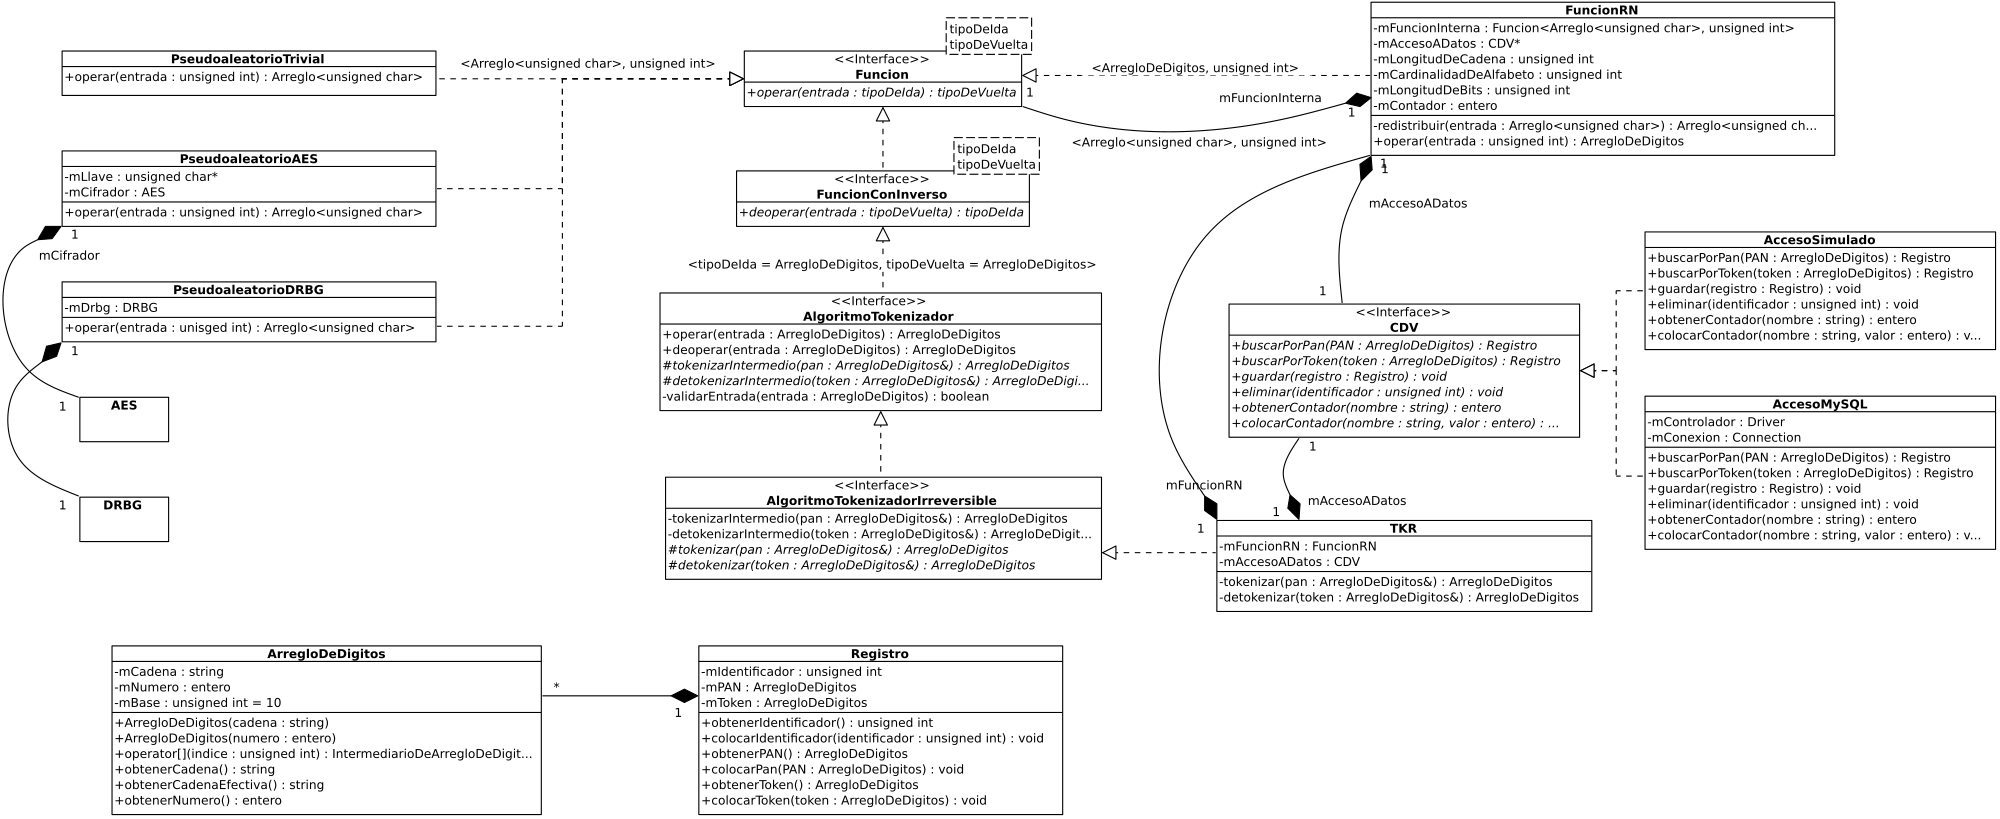
\includegraphics[width=1.0\linewidth]{diagramas/tkr.png}
    \caption{Diagrama de clases de módulo de TKR.}
    \label{clases_tkr}
  \end{center}
\end{sidewaysfigure}
